\documentclass[a4paper,12pt]{article}
\usepackage{outline}
\usepackage{pmgraph}
\usepackage[normalem]{ulem}
\usepackage{comment} % enables the use of multi-line comments (\ifx \fi)
\usepackage{lipsum} %This package just generates Lorem Ipsum filler text.
\usepackage{fullpage} % changes the margin
\usepackage{listings}
\usepackage{color}
\usepackage{mdframed}
\usepackage{listings}
\usepackage{graphicx}
\graphicspath{ {../} }
\renewcommand{\lstlistingname}{Code Block}% Listing -> Algorithm
\renewcommand{\lstlistlistingname}{List of \lstlistingname s}% List of Listings -> List of Algorithms
\title{\textbf{Lab 08: Introduction to Sequential Logic}
\author{Joseph Martinsen \\ ECEN 248-510 \\ TA: Michael Bass}
\date{\today}

\linespread{1.5}
%--------------------Indention
\setlength{\parindent}{15pt}
\lstset{frame=shadowbox, rulesepcolor=\color{white}}
\mdfsetup{frametitlealignment=\center}
\lstset{
  numbers=left,
  stepnumber=1,
  firstnumber=1,
  numberfirstline=true
}

\begin{document}
\section*{Objective}

\hspace{15pt}In this lab, students were introduced to latches and flip-flops. These sequential logic
circuits will be described in first structual Verilog and then behavioral Verilog.
Synchronous sequential circuits will also be introduced towards the end of the lab.
Delays will also be added to logic gates for the first time while implementing a
clock signal. Finally, students will design one block of code that will include
both flip-flops and combinational logic (full adder) to simulate synchronous logic.

\section*{Design}

% Verilog code template
% \lstinputlisting[language=Verilog,,caption=4-Bit ALU ]{../code name.v}

\section*{Results}

Explain the 2 unit delay to 4 units and explain the results of the simulation
(Experiment 1 1.e) \\

(Experiment 1 3.b) Do the latches behave as expected? Why or why not? \\

(Experiment 1 4.b) Compare the waveforms you captured from the behavioral Verilog
to those captured from the structual. Are they different? If so, how?

% Figure with caption
% \begin{figure}[h]
%   \begin{center}
%     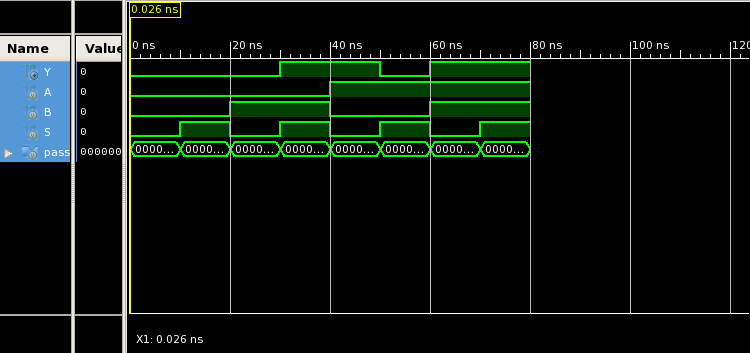
\includegraphics[scale=1]{2_1MuxPlot.png}
%     \caption{\textit{2-Bit 2:1 MUX Plots}}
%   \end{center}
% \end{figure}


\section*{Conclutions}


\section*{Questions}

\begin{enumerate}
  \item \textbf{Include the source code with comments for all modules you
    simulated. You do not have to include test bench code that was
    provided; however, you must supply the test bench code that you wrote! Code
    without comments will not be accepted.}

    \textit{In the report.}

  \item \textbf{Include screenshots of all waveforms captured during simulatio in addition
    to the test bench console output for each test bench simulation.}

    \textit{In the report.}

  \item \textbf{Answer \underline{all} questions throughout the lab manual.}

    \textit{In the report.}

  \item \textbf{Compare the behavioral description of the synchronous adder found in the
    test bench code with the combination of stuctual and dataflow Verilog you
    used in the lab assignment. What are the advantages and disadvantages of each?
    Which do you perfer and why?}

  \item \textbf{Based on the clock period you measured for your synchronous adder, what
    would be the theoretical maximum clock rate? What would be the effect of
    increasing the width of the adder on the clock rate? How might you improve the
    clock rate of the design?}
\end{enumerate}

\section*{Student Feedback}

\begin{enumerate}
  \item \textbf{What did you like most about the lab assignment and why? What did you like least aboub it and why?}
  \vspace{10pt}

  \item \textbf{Were there any section of the lab manual that were unclear? If so, what was unclear? Do you have any suggetions for improving the clarity?}
  \vspace{10pt}

  \item \textbf{What suggestions do you have to improve the overall alb assignment?}
  \vspace{10pt}

\end{enumerate}

\ifx
\begin{thebibliography}{1}
\bibitem{Verilog} Charles Kime \& Thomas Kaminski  \emph{Logic and Computer Design Fundamentals} \\ \hspace{15pt}\textit{http://www.cs.bilkent.edu.tr/~will/courses/CS223/Verilog/LCDF3_Verilog_Ch_4.pdf}
\end{thebibliography}

\section*{Attachments}
%Make sure to change these
Lab Notes, HelloWorld.ic, FooBar.ic
%\fi %comment me out

\begin{thebibliography}{9}
\bibitem{Verilog} Charles Kime & Thomas Kaminski  \emph{Logic and Computer Design Fundamentals} \textit{http://www.cs.bilkent.edu.tr/~will/courses/CS223/Verilog/LCDF3_Verilog_Ch_4.pdf}
\end{thebibliography}

%How to cite
Put your Problem statement here! Example of a Citation\cite[p.219]{Robotics}. Here's Another Citation\cite{Flueck}
\fi
\end{document}
